\documentclass{report}
\usepackage[margin=1in, paperwidth=8.5in, paperheight=11in]{geometry}
%Math packages%
\usepackage{amsmath}
\usepackage{amsthm}
%Spacing%
\usepackage{setspace}
\onehalfspacing
%Lecture number%
\newcommand{\lectureNum}{6}
%Variables - Date and Course%
\newcommand{\curDate}{January 19, 2017}
\newcommand{\course}{CS 251}
\newcommand{\instructor}{Stephen Mann}
%Defining the example tag%
%\theoremstyle{definition}%
\newtheorem{ex}{Example}[section]
%Setting counter given the lecture number%
\setcounter{chapter}{\lectureNum{}}
%Package to insert code%
\usepackage{listings}
\usepackage{courier}
\usepackage{xcolor}
\lstset { %
    tabsize=2,
    breaklines=true,
    language=C++,
    backgroundcolor=\color{blue!8}, % set backgroundcolor
    basicstyle=\footnotesize\ttfamily,% basic font setting
}
%Package used to draw circuits%
\usepackage{circuitikz}
\begin{document}
%Note title%
\begin{center}
\begin{Large}
\textsc{\course{} | Lecture \lectureNum{}}
\end{Large}
\end{center} 
\noindent \textit{Bartosz Antczak} \hfill
\textit{Instructor: \instructor{}} \hfill
\textit{\curDate{}}
\rule{\textwidth}{0.4pt}
% Actual Notes%
\section{Extending the Traffic Light Controller}
Recall in the last lecture, we implemented a basic traffic light controller using a finite-state controller. Let's expand on this implementation by including a timer to change the lights and also a yellow light (rather than just green and red). The graphical representation looks like:
\begin{figure}[ht]
\begin{center}
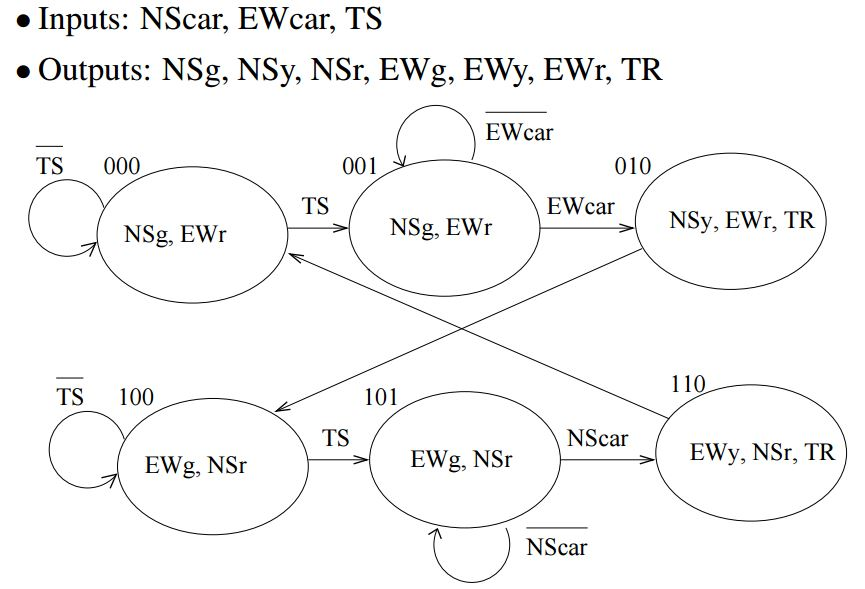
\includegraphics[scale=0.5]{graphical_representation1.jpg}
\end{center}
\caption{Courtesy of Prof. Mann's slides.}
\end{figure}\\
To analyse this diagram, we are given a particular input (which are listed in the diagram) and a current state (that's what the three binary string digits around each bubble represent). Based on the sequence of inputs, we can determine the state of each output (the outputs are listed in the diagram). From this diagram, we can construct the next-state table (on the next page):
\begin{figure}[ht]
\begin{center}
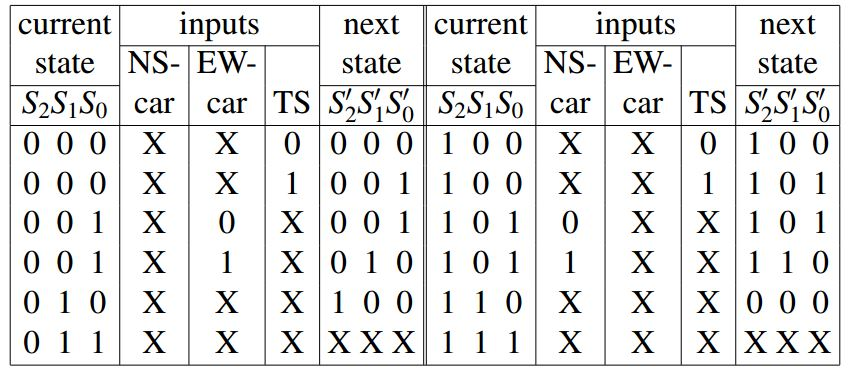
\includegraphics[scale=0.3]{next-state-table-extended.jpg}
\end{center}
\caption{Courtesy of Prof. Mann's slides.}
\end{figure}
\newpage\noindent From this table, we can construct the circuit diagram by analysing the unreduced sums of products for the output logic:
\begin{figure}[ht]
\begin{center}
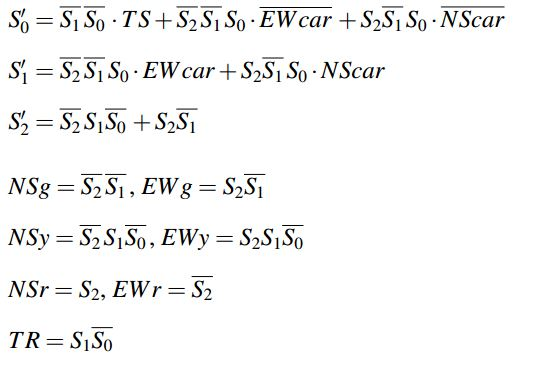
\includegraphics[scale=0.5]{output-logic.jpg}
\end{center}
\caption{The output logic written as an unreduced sums of products. Courtesy of Prof. Mann's slides.}
\end{figure}

\begin{figure}[ht]
\begin{center}
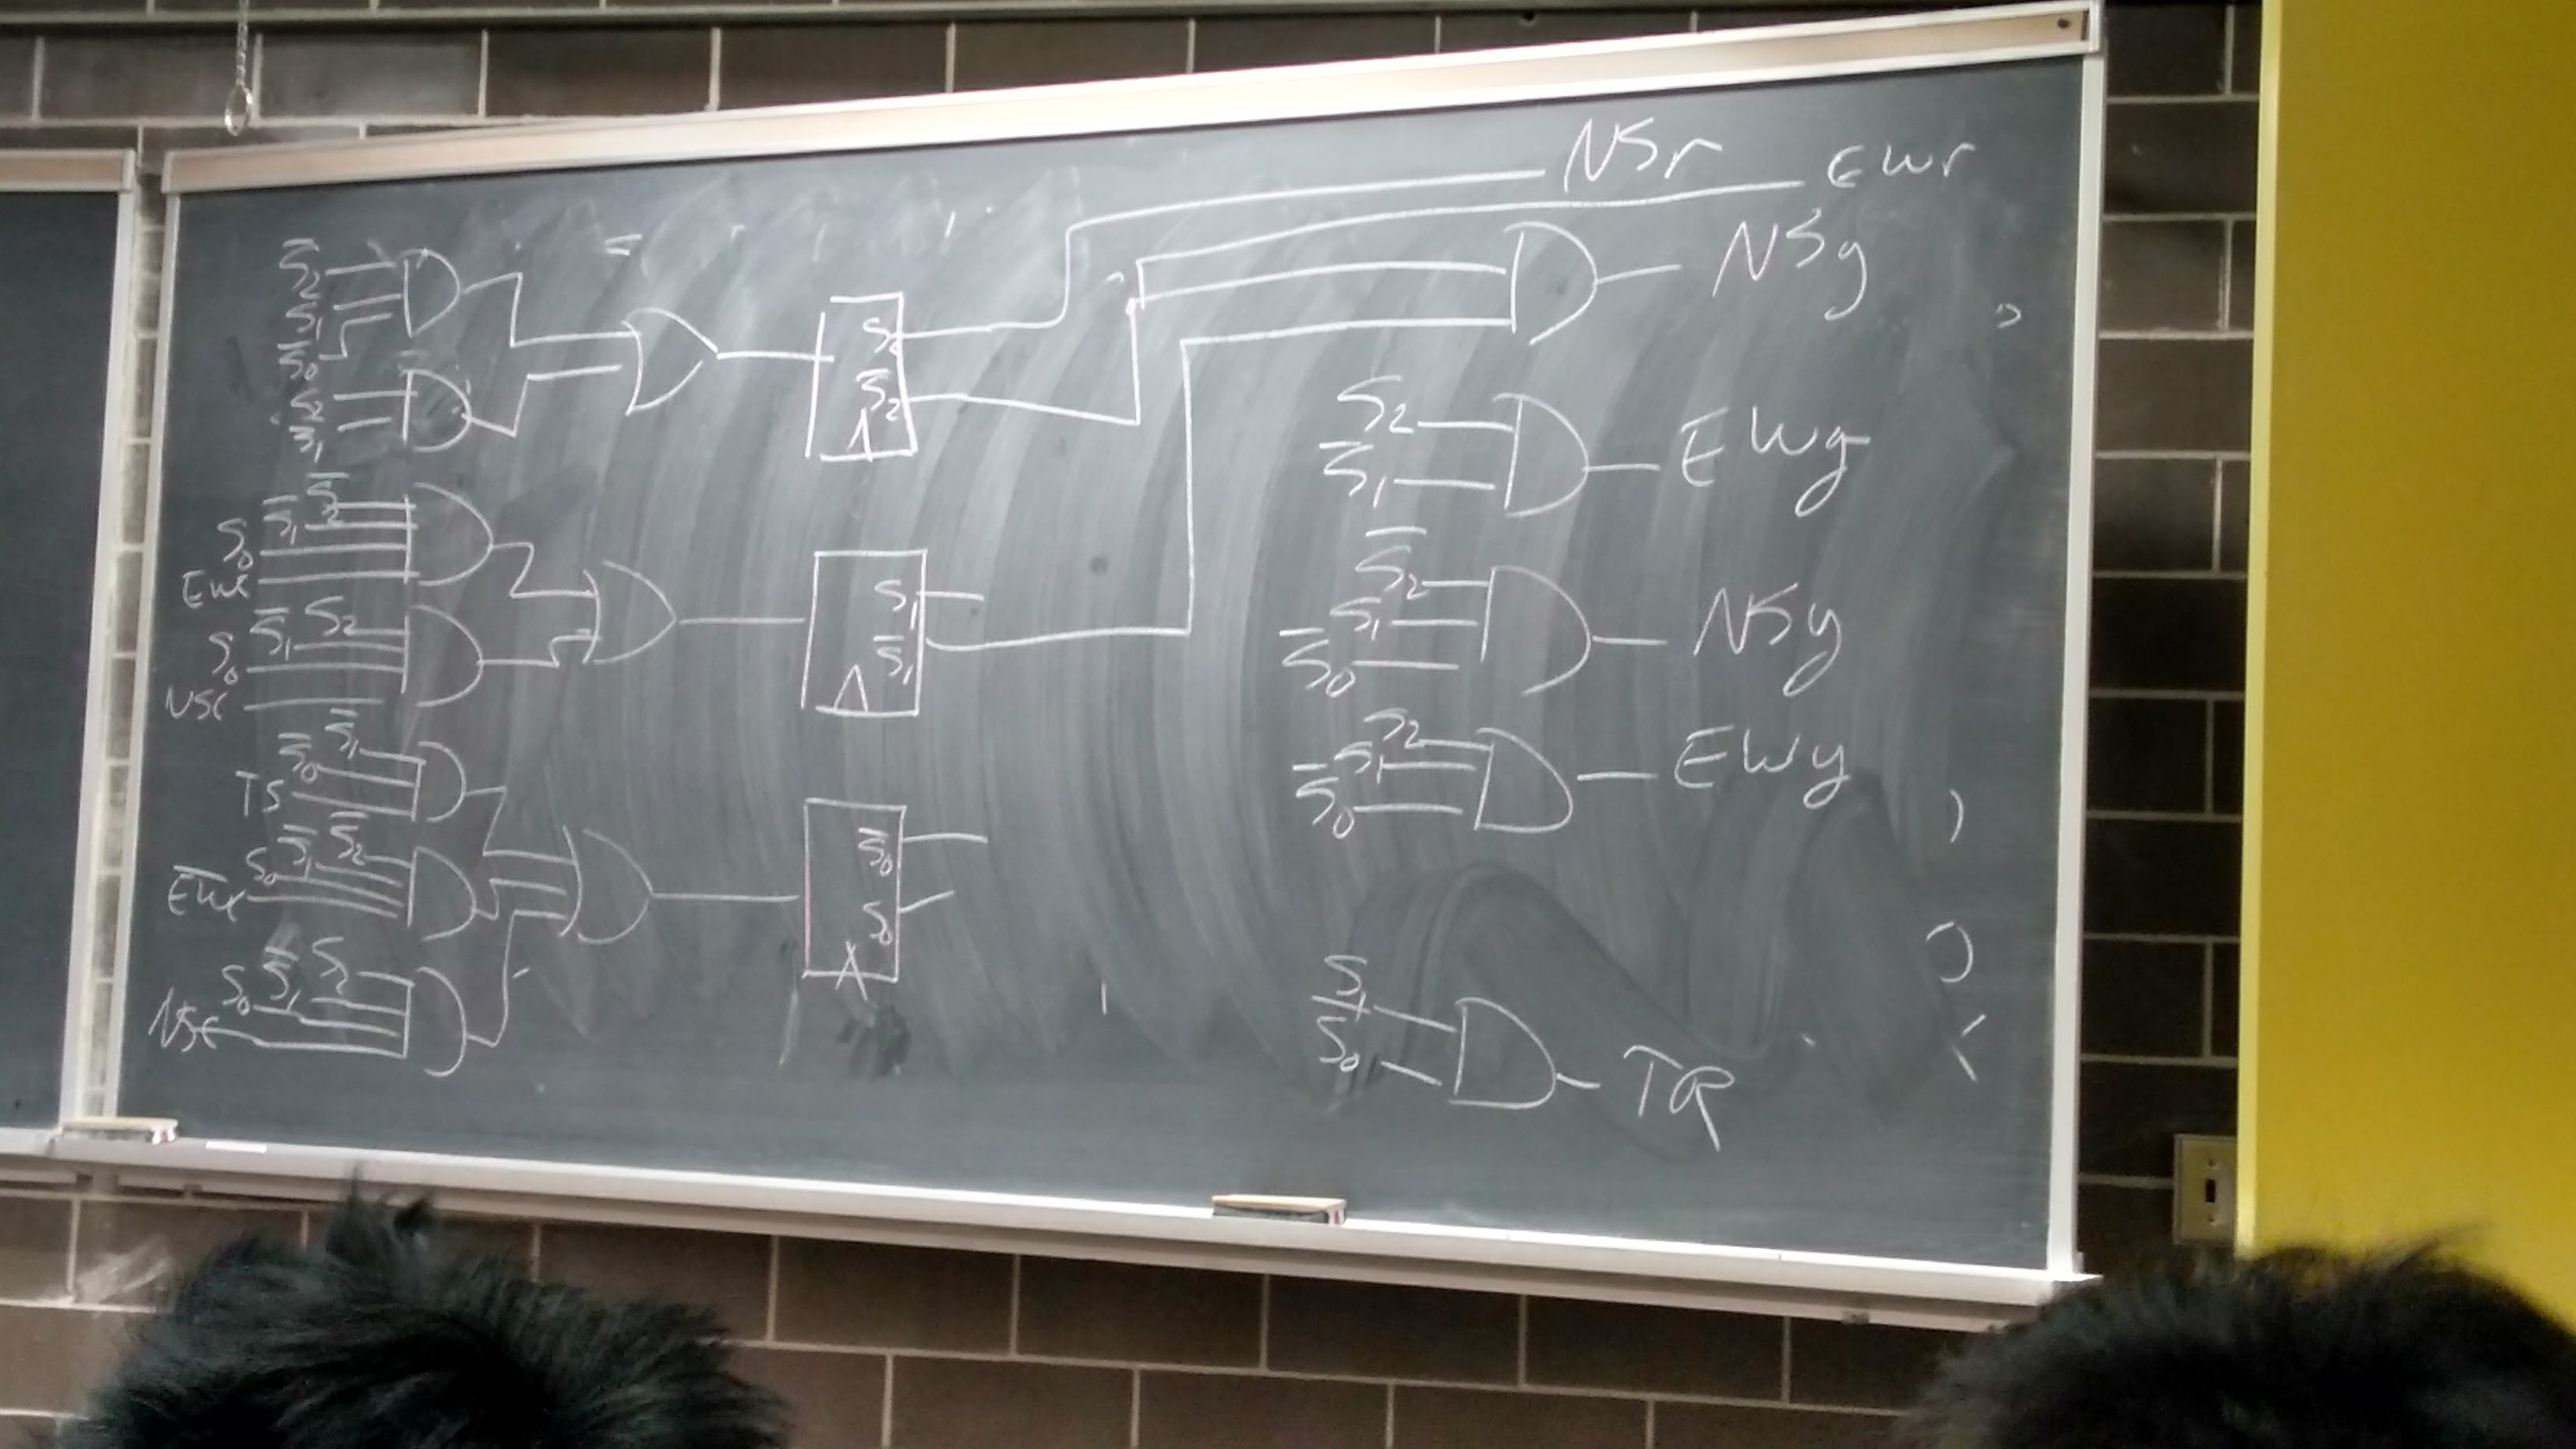
\includegraphics[scale=0.14]{circuit-diagram.jpg}
\end{center}
\caption{Source: Prof. Mann's drawing during today's lecture. It represents the circuit diagram constructed based on the output logic}
\end{figure}

%D flip-fops only store the state input%
\newpage
\section{Data Representation and Manipulation}
\textit{Similar notes are found in my CS 241 course notes ;)}
\subsection{Recall MIPS}
MIPS is an assembly language, which is what high-level language gets compiled into. MIPS then gets compiled to machine code. In CS 251, we're focusing on the MIPS 32-bit architecture, which means that every MIPS word is 32 bits (or 4 bytes) long (i.e., every MIPS instruction represents a binary string that is 32 digits long).
\subsection{Character Representation}
ASCII (American Standard Code for Information Interchange) is a standard that assigns numerical values to characters. For instance, the number 32 (in base-10) represents a space. 97 represents a lower-case `a". ASCII only represents American characters, so to account for the other accents and letter from languages all over the world, \textit{unicode} was standardized.
\begin{center}
\textit{We'll continue more on this topic in the next lecture}
\end{center}
%END%
\end{document}